% Copyright 2018-2023 Pietro Prandini
%
% This file is part of GuitarHub.
%
% GuitarHub is free software: you can redistribute it and/or modify
% it under the terms of the GNU General Public License as published by
% the Free Software Foundation, either version 3 of the License, or
% (at your option) any later version.
%
% GuitarHub is distributed in the hope that it will be useful,
% but WITHOUT ANY WARRANTY; without even the implied warranty of
% MERCHANTABILITY or FITNESS FOR A PARTICULAR PURPOSE.  See the
% GNU General Public License for more details.
%
% You should have received a copy of the GNU General Public License
% along with GuitarHub.  If not, see <https://www.gnu.org/licenses/>.

% \begin{titlepage}
% 	\vspace*{\stretch{6}}
% 	 \begin{center}
% 	 	{\ttfamily\huge\bfseries Pietro e Maria\par}
% 	 %\end{center}
% 	%\vspace*{\stretch{1}}
% 	%\begin{center}
% 		{\ttfamily\scshape\Large 11 - 06 - 2022\par}
%  	  \vspace*{\stretch{1}}
%     {\ttfamily\scshape\normalsize Canti\par}
% 	%\end{center}
% 	\vspace*{\stretch{2}}
% 	%\begin{center}
% 		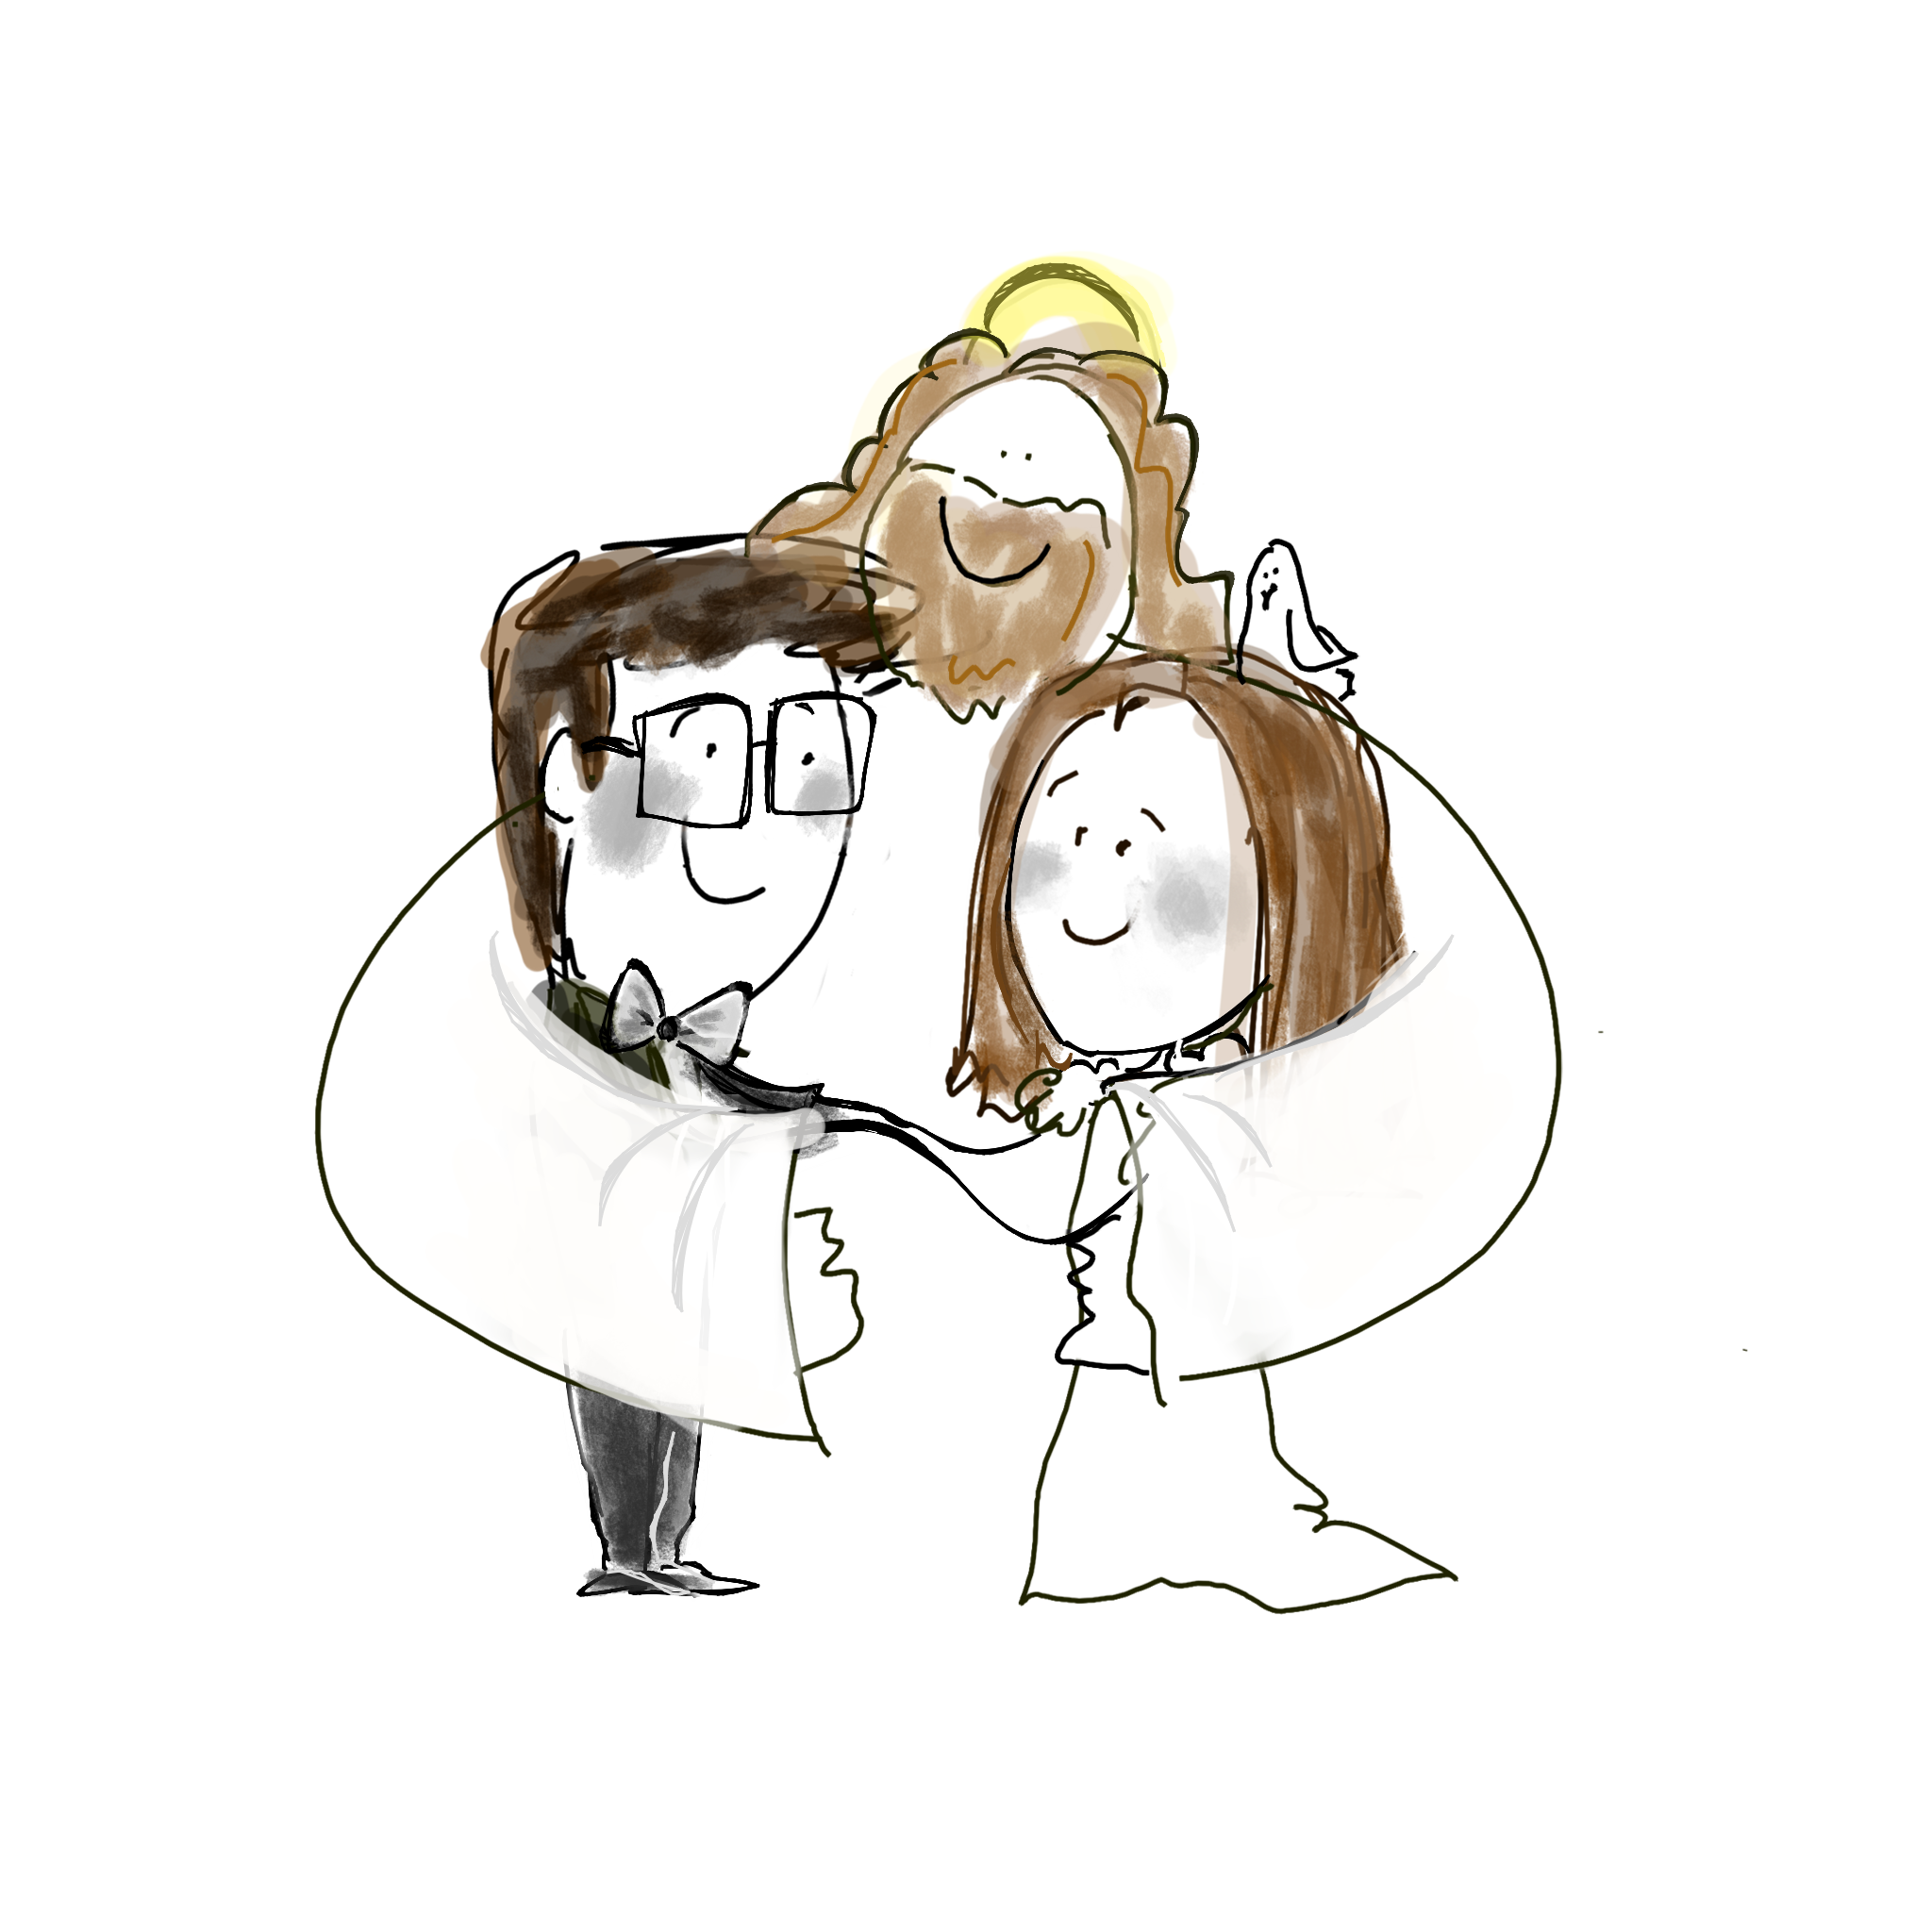
\includegraphics[width=11cm]{img/DMP}\\ % GitHub picture
% 		%{\ttfamily\footnotesize \href{https://github.com/PietroPrandini/GuitarHub}{https://github.com/PietroPrandini/GuitarHub}\par}
% 		%\medskip
% 		%\qrcode[hyperlink,height=1.5cm]{https://github.com/PietroPrandini/GuitarHub}
% 	\end{center}
% 	\vspace*{\stretch{8}}
% \end{titlepage}
